%%%%%%%%%%%%%%%%%%%%%%%%%%%%%%%%%%%%%%%%%%%%%%%%%%%%%%
% From Vibe Coding to Spec-Driven Development        %
% Beamer slide deck (UTU theme, 16:9)                %
%%%%%%%%%%%%%%%%%%%%%%%%%%%%%%%%%%%%%%%%%%%%%%%%%%%%%%

\documentclass[aspectratio=169]{beamer}
\usepackage{hyperref}
\usepackage[T1]{fontenc}

% core packages
\usepackage{latexsym,amsmath,amssymb,xcolor,multicol,booktabs}
\usepackage{graphicx,listings}

\author{Cuong Kane}
\title[Vibe Coding to SDD]{From Vibe Coding to Spec-Driven Development}
\subtitle{How SDD is re-emerging as a critical methodology for AI-assisted development}
\institute{cuongkane.com}
\date{April 2026}

\usepackage{UTU}

% convenience macros
\def\cmd#1{\texttt{\color{red}\footnotesize $\backslash$#1}}
\def\env#1{\texttt{\color{blue}\footnotesize #1}}
\definecolor{utu_green}{RGB}{173,203,0}
\definecolor{utu_blue}{RGB}{93,155,162}
\definecolor{utu_pink}{RGB}{248,72,94}
\definecolor{halfgray}{gray}{0.55}
\definecolor{lightgray}{gray}{0.9}

\lstset{
    basicstyle=\ttfamily\small,
    keywordstyle=\bfseries\color{utu_green},
    emphstyle=\ttfamily\color{utu_blue},
    stringstyle=\color{utu_pink},
    numbers=left,
    numberstyle=\small\color{halfgray},
    rulesepcolor=\color{red!20!green!20!blue!20},
}

\begin{document}

% ============================================================
% TITLE
% ============================================================
\begin{frame}
    {\small \titlepage}
\end{frame}

% ============================================================
\section{Context}
% ============================================================

\begin{frame}{AI Has Changed How We Code}
    In 2026, AI coding tools are part of every developer's daily workflow.

    \vspace{0.4cm}
    \begin{itemize}
        \item \textbf{``Vibe coding''} has entered the mainstream -- prompt and let the AI handle the rest
        \item LLMs can now implement most technical tasks \textbf{autonomously}
        \item The developer's role has shifted: less writing code, more \textbf{directing and reviewing}
    \end{itemize}

    \vspace{0.5cm}
    \colorbox{utu_blue!20}{\parbox{0.9\textwidth}{
        \centering
        \textbf{The bottleneck is no longer typing speed -- it's clarity of intent.}
    }}
\end{frame}

\begin{frame}{The New Developer Role}
    \vspace{0.3cm}
    \begin{columns}[T]
        \begin{column}{0.45\textwidth}
            \colorbox{utu_green!20}{\parbox{0.95\textwidth}{\centering\textbf{AI is great at}}}
            \vspace{0.3cm}
            \begin{itemize}
                \item \textit{How} to build something
                \item Generating code fast
                \item Following patterns
                \item Repetitive tasks
            \end{itemize}
        \end{column}
        \begin{column}{0.45\textwidth}
            \colorbox{utu_pink!20}{\parbox{0.95\textwidth}{\centering\textbf{Humans still own}}}
            \vspace{0.3cm}
            \begin{itemize}
                \item \textit{What} to build and \textit{why}
                \item Defining requirements
                \item Validating correctness
                \item Business judgment
            \end{itemize}
        \end{column}
    \end{columns}
\end{frame}

% ============================================================
\section{Problem Statement}
% ============================================================

\begin{frame}{The Hidden Cost of AI Speed}
    Teams relying heavily on AI coding agents consistently hit four problems:

    \vspace{0.5cm}
    \begin{columns}[T]
        \begin{column}{0.45\textwidth}
            \colorbox{utu_pink!20}{\parbox{0.95\textwidth}{\centering\textbf{1. Quality at scale}}}
            \vspace{0.15cm}
            {\small Code generated faster than teams can review}

            \vspace{0.4cm}
            \colorbox{utu_pink!20}{\parbox{0.95\textwidth}{\centering\textbf{2. Redundant loops}}}
            \vspace{0.15cm}
            {\small Costly prompt-review-correct cycles}
        \end{column}
        \begin{column}{0.45\textwidth}
            \colorbox{utu_pink!20}{\parbox{0.95\textwidth}{\centering\textbf{3. Token consumption}}}
            \vspace{0.15cm}
            {\small AI ingests too much context, diminishing returns}

            \vspace{0.4cm}
            \colorbox{utu_pink!20}{\parbox{0.95\textwidth}{\centering\textbf{4. Code is a liar}}}
            \vspace{0.15cm}
            {\small AI replicates bad patterns from accidental behavior}
        \end{column}
    \end{columns}
\end{frame}

\begin{frame}{Quality at Scale}
    \begin{itemize}
        \item AI produces hundreds of lines in minutes
        \item Verifying correctness still requires \textbf{human judgment}
        \item Without a shared spec, code review becomes a \textbf{bottleneck} -- or a rubber stamp
    \end{itemize}

    \vspace{0.5cm}
    \colorbox{utu_pink!20}{\parbox{0.9\textwidth}{
        \centering
        \textbf{Speed without direction creates technical debt faster than ever.}
    }}
\end{frame}

\begin{frame}{The Redundant Loop}
    Without a clear spec, developers fall into a costly refinement cycle:

    \vspace{0.4cm}
    \begin{enumerate}
        \item \textbf{Prompt:} ``create a button in the center''
        \item \textbf{AI:} creates it too big with ugly centering
        \item \textbf{Prompt:} ``no, I need...''
        \item Repeat \textbf{dozens of times} per feature
    \end{enumerate}

    \vspace{0.5cm}
    \colorbox{utu_green!20}{\parbox{0.9\textwidth}{
        \centering
        \textbf{A clear spec upfront eliminates most of these rounds.}
    }}
\end{frame}

\begin{frame}{Token Waste \& Code as a Liar}
    \begin{columns}[T]
        \begin{column}{0.45\textwidth}
            \colorbox{utu_blue!20}{\parbox{0.95\textwidth}{\centering\textbf{Token Consumption}}}
            \vspace{0.3cm}
            \begin{itemize}
                \item AI reads entire repo to understand behavior
                \item Codebases are poorly structured for machines
                \item Heavy token use, diminishing returns
            \end{itemize}
        \end{column}
        \begin{column}{0.45\textwidth}
            \colorbox{utu_blue!20}{\parbox{0.95\textwidth}{\centering\textbf{Code is a Liar}}}
            \vspace{0.3cm}
            \begin{itemize}
                \item Dead code, redundant complexity
                \item AI hallucinates intent from accidental behavior
                \item Specs capture \textit{intended}, not \textit{accidental}
            \end{itemize}
        \end{column}
    \end{columns}
\end{frame}

% ============================================================
\section{SDD Solution}
% ============================================================

\begin{frame}{What is Spec-Driven Development?}
    \begin{itemize}
        \item \textbf{SDD} = write a detailed requirement specification \textit{before} writing code
        \item Not new -- Microsoft introduced it in the early 2000s
        \item Most familiar example: \textbf{API-first development} (OpenAPI spec as contract)
    \end{itemize}

    \vspace{0.5cm}
    \colorbox{utu_blue!20}{\parbox{0.9\textwidth}{
        \centering
        \textbf{In 2026, SDD is re-emerging because the developer's primary job\\has shifted from writing code to writing and clarifying requirements.}
    }}
\end{frame}

\begin{frame}{Level 1: Spec-First}
    \begin{itemize}
        \item Spec is written \textbf{before} implementation to guide initial development
        \item Once code exists, spec may or may not be maintained
        \item Best for: \textbf{prototypes, POCs}, projects that won't be maintained long-term
    \end{itemize}

    \vspace{0.5cm}
    \colorbox{utu_green!20}{\parbox{0.9\textwidth}{
        \centering
        \textbf{Forces upfront clarity, even if the spec becomes disposable.}
    }}
\end{frame}

\begin{frame}{Level 2: Spec-Anchored}
    \begin{itemize}
        \item Spec is maintained \textbf{alongside the code} throughout the system's lifecycle
        \item Changes to behavior require updating \textbf{both} spec and code
        \item AI reads the spec instead of reverse-engineering intent from the codebase
        \item Tests follow the spec strictly and validate against source code
    \end{itemize}

    \vspace{0.5cm}
    \colorbox{utu_green!20}{\parbox{0.9\textwidth}{
        \centering
        \textbf{Best fit for most modern software teams using AI agents.}
    }}
\end{frame}

\begin{frame}{Level 3: Spec-as-Source}
    \begin{itemize}
        \item Spec is the \textbf{only artifact} humans edit directly
        \item Code is entirely \textbf{generated} from the spec -- never manually modified
        \item Requires mature code generation tooling and comprehensive automated tests
    \end{itemize}

    \vspace{0.3cm}
    \colorbox{utu_green!20}{\parbox{0.9\textwidth}{
        \centering
        \textbf{Spec becomes the single source of truth; codebase stays deterministic.}
    }}

    \vspace{0.2cm}
    \colorbox{utu_pink!20}{\parbox{0.9\textwidth}{
        \centering
        \textbf{A higher level doesn't always mean better. Start where your team is ready.}
    }}
\end{frame}

\begin{frame}{Three Levels of SDD}
    \begin{figure}[htpb]
        \centering
        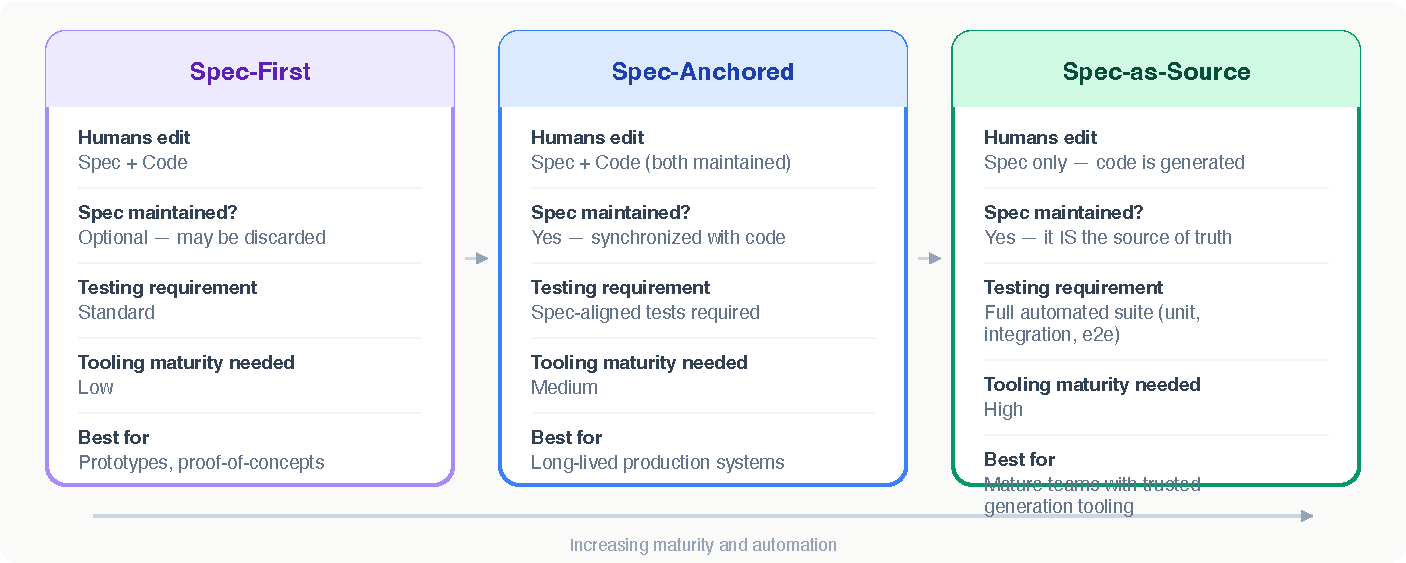
\includegraphics[keepaspectratio, width=0.85\textwidth, height=0.75\textheight]{fig/sdd_levels.pdf}
    \end{figure}
\end{frame}

% ============================================================
\section{SDD Workflow}
% ============================================================

\begin{frame}{A Typical SDD Workflow}
    Three phases: \textbf{Constitution}, \textbf{Feature Development}, and \textbf{Replanning}.

    \vspace{0.3cm}
    \begin{figure}[htpb]
        \centering
        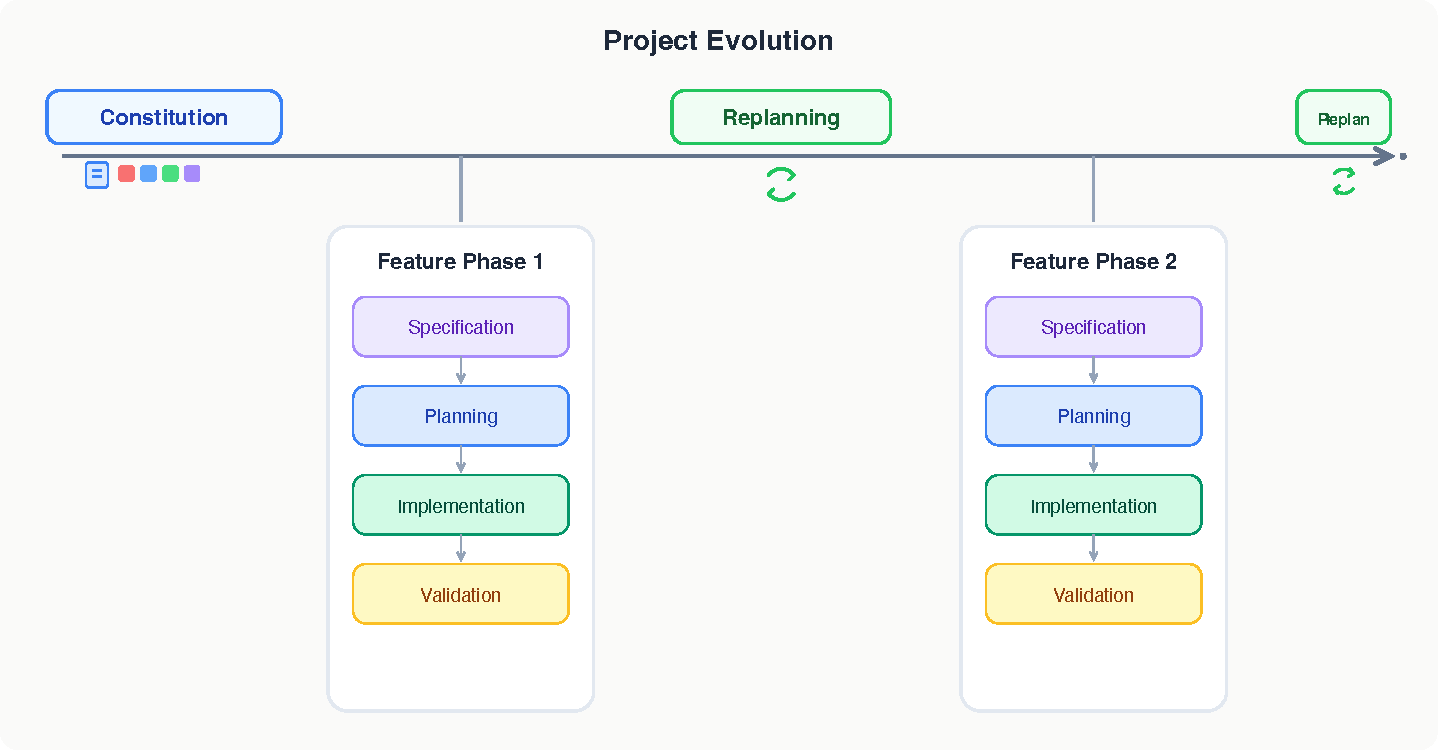
\includegraphics[keepaspectratio, width=0.85\textwidth]{fig/workflow.pdf}
    \end{figure}
\end{frame}

\begin{frame}{Phase 1: Constitution}
    Define the high-level foundation for your project:

    \vspace{0.4cm}
    \begin{columns}[T]
        \begin{column}{0.45\textwidth}
            \colorbox{utu_green!20}{\parbox{0.95\textwidth}{\centering\textbf{Greenfield}}}
            \vspace{0.3cm}
            \begin{itemize}
                \item Project goal
                \item Tech stack
                \item Roadmap
            \end{itemize}
        \end{column}
        \begin{column}{0.45\textwidth}
            \colorbox{utu_blue!20}{\parbox{0.95\textwidth}{\centering\textbf{Brownfield}}}
            \vspace{0.3cm}
            \begin{itemize}
                \item Read existing codebase
                \item Build initial specification
                \item Capture project purpose
            \end{itemize}
        \end{column}
    \end{columns}

    \vspace{0.4cm}
    \colorbox{utu_blue!20}{\parbox{0.9\textwidth}{
        \centering
        \textbf{Outcome: living documentation as the entry point for humans and AI.}
    }}
\end{frame}

\begin{frame}{Phase 2: Feature Development}
    Each new feature follows four steps:

    \vspace{0.4cm}
    \begin{enumerate}
        \item \textbf{Specification} -- clarify requirements, use Gherkin format for acceptance criteria
        \item \textbf{Planning} -- write implementation plan (architecture, boundaries, data flow)
        \item \textbf{Implementation} -- break into smaller tasks, feed to AI agent with tests
        \item \textbf{Validation} -- run tests; if they fail, fix code or correct spec (human decision)
    \end{enumerate}
\end{frame}

\begin{frame}{Phase 3: Replanning}
    \begin{itemize}
        \item No plan survives first contact with code
        \item \textbf{Replanning} = updating the spec to reflect what was learned
        \item Keeps spec and code synchronized rather than drifting apart
        \item Can be triggered by AI, but always requires \textbf{human approval}
    \end{itemize}

    \vspace{0.5cm}
    \colorbox{utu_blue!20}{\parbox{0.9\textwidth}{
        \centering
        \textbf{This feedback loop is also known as ``harness engineering.''}
    }}
\end{frame}

\begin{frame}{The Human Factor}
    \vspace{0.3cm}
    \begin{figure}[htpb]
        \centering
        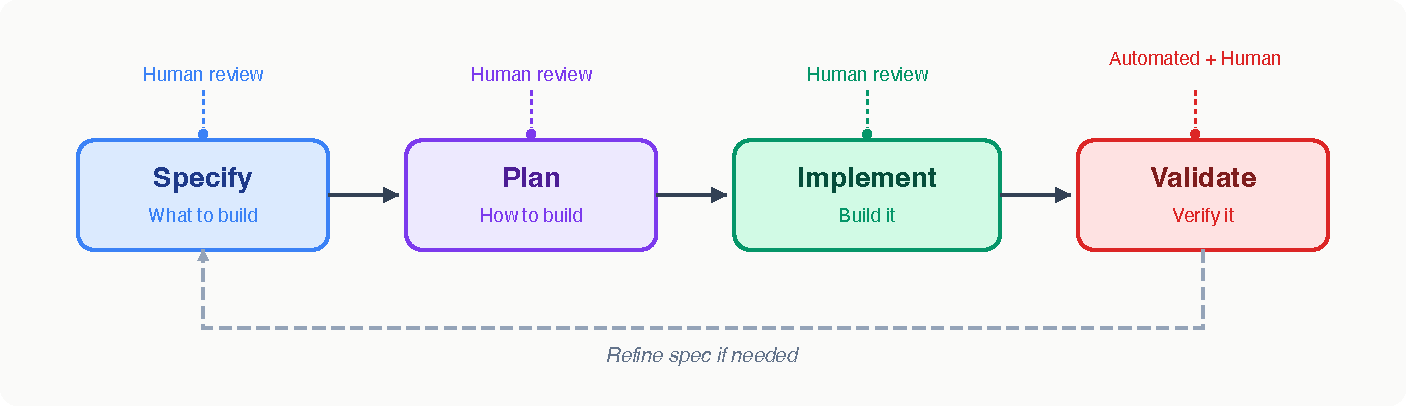
\includegraphics[keepaspectratio, width=0.95\textwidth]{fig/human_factor.pdf}
    \end{figure}
    \vspace{0.3cm}
    {\small Replanning happens after code review when requirements change -- always with \textbf{human approval}.}
\end{frame}

% ============================================================
\section{Adopting SDD in Practice}
% ============================================================

\begin{frame}{SDD Tools Landscape (April 2026)}
    \vspace{0.2cm}
    \begin{center}
        \small
        \begin{tabular}{l l l l}
            \toprule
            \textbf{Tool} & \textbf{Best fit} & \textbf{Complexity} & \textbf{Workflow style} \\
            \midrule
            Spec Kit & Structured checkpoints & Medium & specify $\to$ plan $\to$ implement \\
            BMAD & Enterprise, multi-role & High & Multi-agent personas \\
            OpenSpec & Brownfield, fast iteration & Low & propose $\to$ apply $\to$ archive \\
            Kiro & AWS-native, IDE integration & Medium & Integrated IDE pipeline \\
            \bottomrule
        \end{tabular}
    \end{center}

    \vspace{0.4cm}
    \begin{itemize}
        \item Spec Kit, BMAD, OpenSpec are \textbf{agent-agnostic} (Claude, Copilot, Cursor, etc.)
        \item Kiro is tied to AWS Bedrock but offers the most integrated experience
    \end{itemize}
\end{frame}

\begin{frame}{SDD Reshapes the SDLC}
    \begin{columns}[T]
        \begin{column}{0.42\textwidth}
            \vspace{0.3cm}
            {\small SDD doesn't replace the SDLC -- it reshapes it:}
            \vspace{0.2cm}
            \begin{itemize}
                \item {\small Requirements $\to$ spec authoring}
                \item {\small Design $\to$ planning with AI}
                \item {\small Implementation $\to$ AI-driven generation}
                \item {\small QA $\to$ automated spec-based validation}
            \end{itemize}
            \vspace{0.3cm}
            \colorbox{utu_green!20}{\parbox{0.95\textwidth}{
                \centering
                {\small \textbf{Specs are the connective tissue between every phase.}}
            }}
        \end{column}
        \begin{column}{0.55\textwidth}
            \begin{figure}
                \centering
                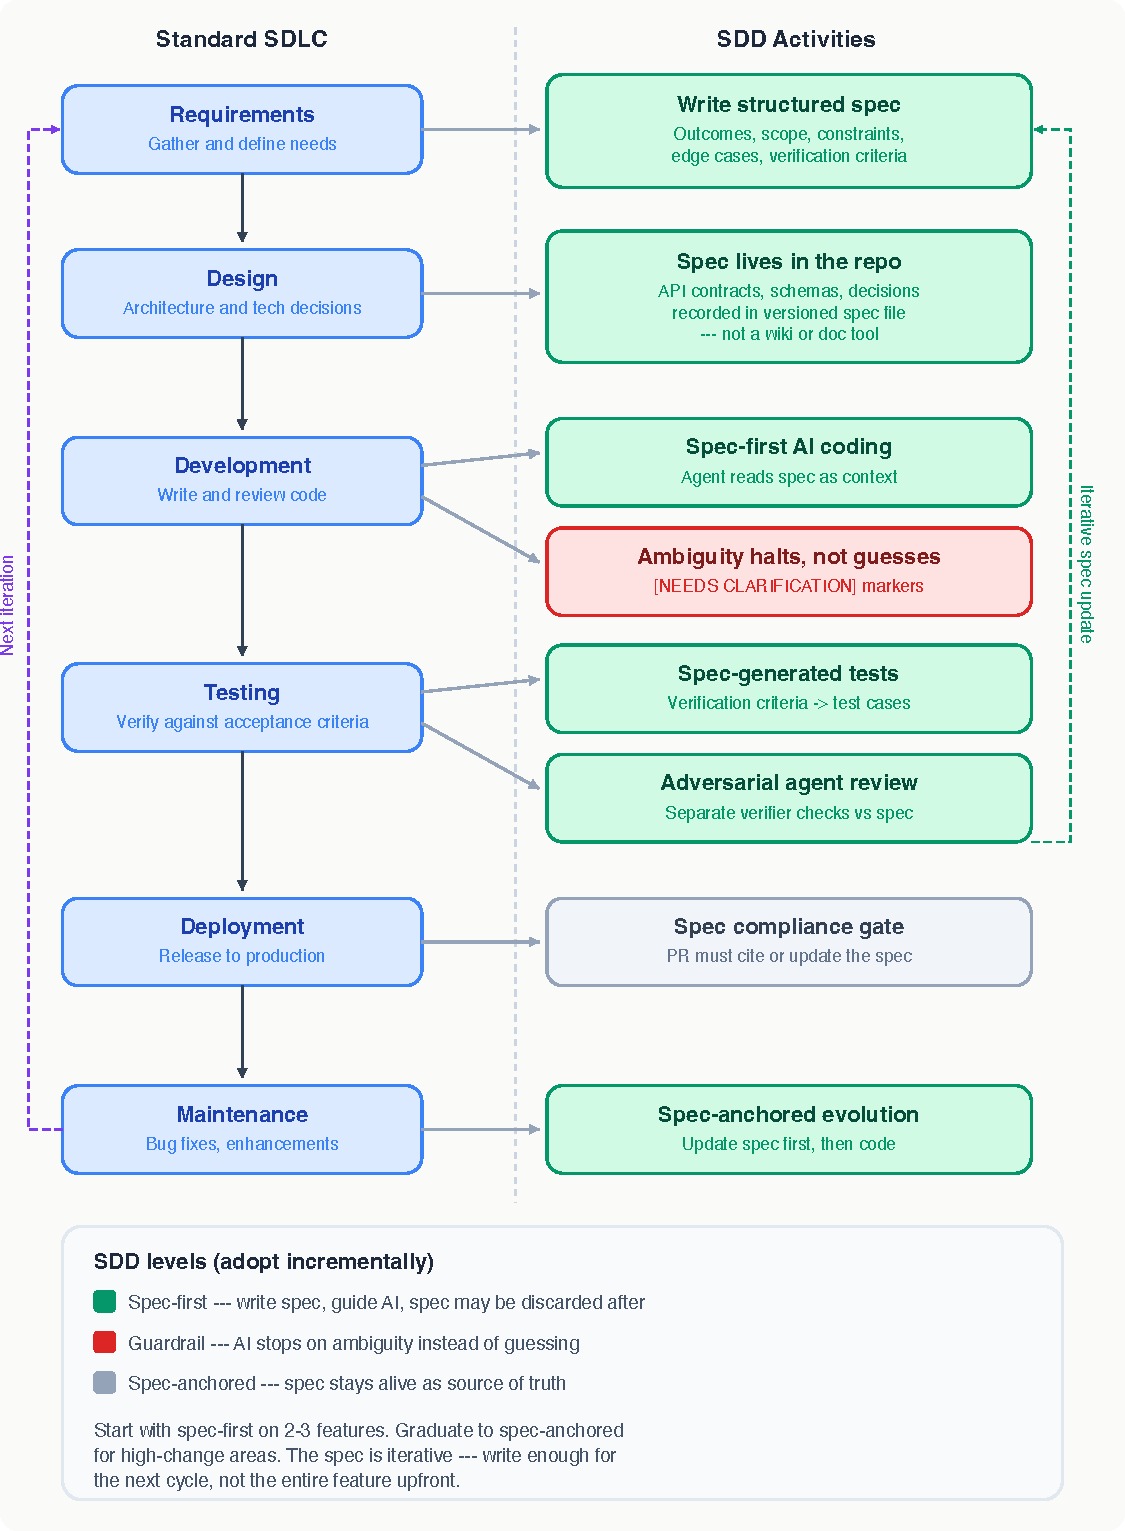
\includegraphics[keepaspectratio, height=0.75\textheight]{fig/sdd_general_sdlc.pdf}
            \end{figure}
        \end{column}
    \end{columns}
\end{frame}

% ============================================================
\section{Conclusion}
% ============================================================

\begin{frame}{Key Takeaways}
    \begin{itemize}
        \item Use \textbf{spec-first} for initial development, \textbf{spec-anchored} for production systems, \textbf{spec-as-source} only when generation tooling is mature

        \vspace{0.2cm}
        \item Traditional design docs are advisory; \textbf{SDD specs are enforced} -- tests fail if code diverges

        \vspace{0.2cm}
        \item Like TDD and BDD, SDD focuses on \textbf{end-user behavior and original intent} before writing code

        \vspace{0.2cm}
        \item Adopting SDD requires setup effort, good automated tests, and a mindset shift to treat the spec as a \textbf{first-class artifact}
    \end{itemize}

    \vspace{0.3cm}
    \colorbox{utu_green!20}{\parbox{0.9\textwidth}{
        \centering
        \textbf{SDD is a sustainable investment for teams building with AI.}
    }}
\end{frame}

\begin{frame}{References}
    {\small
    \begin{itemize}
        \item Spec-Driven Development: From Code to Contract -- Deepak Babu Piskala
        \item Understanding SDD: Kiro, spec-kit, and Tessl -- Martin Fowler
        \item Deeplearning AI -- AI Agentic Workflows
        \item GitHub Spec Kit | OpenSpec | BMAD Method | Kiro
    \end{itemize}
    }
\end{frame}

\begin{frame}
    \begin{center}
        {\Huge\textit{Thank You}}
    \end{center}
\end{frame}

\end{document}
